\section{Application to an e-governance workload}
\label{sec:case}

\subsection{Workload profile}

We instantiate Problem~\ref{prob:sizing} on a national-scale electronic voting
profile: approximately $3.0\times10^{7}$ ballots cast over a twelve-hour
window, which averages to about $7\times10^{2}$ transactions per second, with a
peak window concentrating roughly a quarter of the daily volume and therefore a
peak demand $\Dpk\approx2.1\times10^{3}$ transactions per second. The safety
requirement is that a coordinated omission fault affecting one fifth of the
validators be detected within one epoch with probability at least
$1-\epss$.

\subsection{Sizing}

Substituting the calibrated parameters of Section~\ref{sec:results} and the
measured detector characteristics into Algorithm~\ref{alg:sizing} yields the
feasibility window $[\resNminCase,\resNmaxCase]$ and the recommendation
$\nopt=\resNoptCase$.

\begin{figure}[!t]
\centering
% 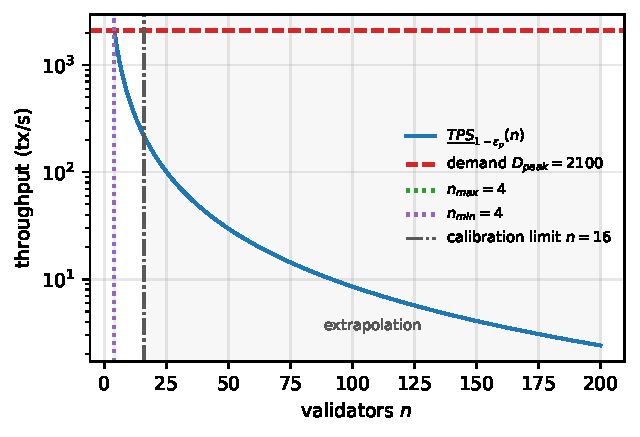
\includegraphics[width=0.8\textwidth]{figures/fig_window}
\rule{0.8\textwidth}{0.24\textwidth}
\caption{Feasibility window. The decreasing curve is the confidence-adjusted
throughput $\underline{\TPS}_{1-\epsp}(\n)$ against the demand $\Dpk$; the
decreasing dashed curve is $\pmiss(\n,\w)$ against the safety target $\epss$.
The admissible interval $[\nmin,\nmax]$ is shaded}
\label{fig:window}
\end{figure}

\subsection{Sensitivity}

The width of the window determines how much design margin the deployment has.
We vary one factor at a time around the calibrated operating point:

\begin{enumerate*}
\item \textbf{Consensus exponent.} A relative change in $\beta$ shifts
$\log\nmax$ by $-\log\nmax\,\Delta\beta/\beta$, so the upper endpoint is most
sensitive precisely when the deployment already sits far above the calibration
range.
\item \textbf{Fault correlation.} Increasing $\rho$ inflates $\nmin$
proportionally to $1+(\kf-1)\rho$ by~\eqref{eq:nmin}; strongly coordinated
faults can close the window on their own.
\item \textbf{Wide-area latency.} Using $\beta(\text{RTT})$ measured in
experiment X4 lowers $\nmax$, quantifying the price of geographic distribution.
\item \textbf{Risk levels.} Tightening $\epsp$ lowers $\nmax$ while tightening
$\epss$ raises $\nmin$; the window therefore closes from both sides as the
system is made more conservative.
\end{enumerate*}

\begin{figure}[!t]
\centering
% 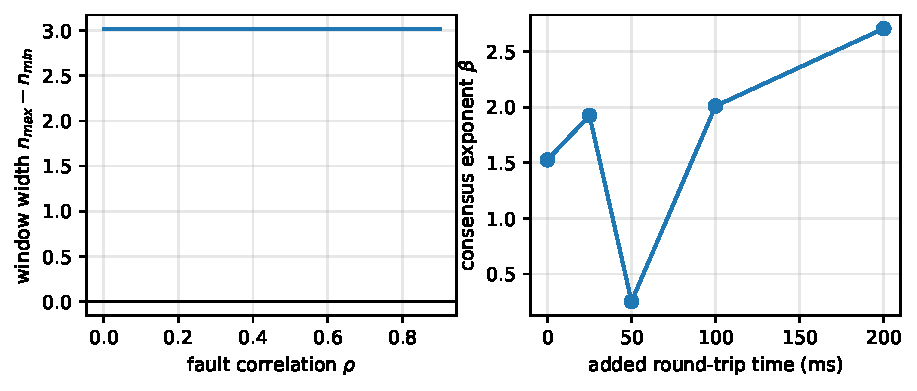
\includegraphics[width=0.8\textwidth]{figures/fig_sensitivity}
\rule{0.8\textwidth}{0.22\textwidth}
\caption{Window width $\nmax-\nmin$ as a function of the fault correlation
$\rho$ and of the added round-trip latency. The zero contour is the
infeasibility boundary of Corollary~\ref{cor:infeasible}}
\label{fig:sensitivity}
\end{figure}

\subsection{Deployment reading}

The analysis produces an operational statement of the form: \emph{with
confidence $1-\epsp$ the network sustains the peak demand for validator counts
up to $\nmax$, and it detects the specified coordinated fault with probability
at least $1-\epss$ for validator counts from $\nmin$ upward; the cheapest
admissible configuration is $\nopt$}. Where the window is empty,
Corollary~\ref{cor:infeasible} states that no choice of validator count
suffices and that the architecture, not the provisioning, must change.

\begin{Remark}
This case study illustrates the sizing workflow. It is not a recommendation to
conduct binding elections on a blockchain: the consensus layer addresses neither
endpoint compromise nor coercion, as established
in~\cite{springall2014,specter2020,park2021}. The same workflow applies
unchanged to registry and identity workloads, where those objections do not
arise.
\end{Remark}
